% This is LLNCS.DEM the demonstration file of
% the LaTeX macro package from Springer-Verlag
% for Lecture Notes in Computer Science,
% version 2.4 for LaTeX2e as of 16. April 2010
%
\documentclass{llncs}
%
\usepackage{makeidx}  % allows for indexgeneration
%



\usepackage[english,activeacute]{babel}
\usepackage[english]{layout}
\usepackage{amsfonts,amssymb}
\usepackage{amsmath}
\usepackage{amsopn} % DeclareMathOperator
\usepackage{amsbsy} % boldsymbol
\usepackage[dvips]{graphicx}
\usepackage{color}
\usepackage{subfig}
\usepackage{colonequals}
\usepackage[latin1]{inputenc}
\usepackage{url}
\usepackage{epsfig}
\usepackage{dsfont}
\usepackage{multirow}

\usepackage{algorithm}
\usepackage{algorithmic}
\usepackage{setspace}
\usepackage{afterpage}
%\usepackage{showkeys}
% \usepackage{mathptmx}      % use Times fonts if available on your TeX system
% \usepackage{latexsym}

%\usepackage[left=1.2in,right=1.2in]{geometry}

% \graphicspath{{../iccv09/}}

\newcommand{\ma}[1]{\boldsymbol{#1}}
\newcommand{\tras}[1]{#1^{\mathrm{T}}}
\newcommand{\herm}[1]{#1^{\mathrm{H}}}
\newcommand{\con}[1]{#1^{\mathrm{*}}}
\newcommand{\E}{\mathds{E}}
\newcommand{\tech}[1]{\overline{#1}}
\newcommand{\nspace}{\!\!\!\!}
\newcommand{\nmbr}[1]{\oldstylenums{#1}}

\newcommand{\eg}{\emph{e.g}. } \newcommand{\Eg}{\emph{E.g}. }
\newcommand{\ie}{\emph{i.e}. } \newcommand{\Ie}{\emph{I.e}. }
\newcommand{\cf}{\emph{c.f}. } \newcommand{\Cf}{\emph{C.f}. }
\newcommand{\etc}{\emph{etc}. } \newcommand{\vs}{\emph{vs}. }
\newcommand{\wrt}{w.r.t\onedot } \newcommand{\dof}{d.o.f. }
\newcommand{\etal}{\emph{et al}. }

\newcommand{\R}{\mathds{R}}
\newcommand{\sign}{\mathrm{sign}}
\newcommand{\eps}{\varepsilon}
\newcommand{\To}{\longrightarrow}
% \newcommand{\II}{1{\hskip -2.5 pt}\hbox{I}}

\newcommand{\best}[1]{\textbf{#1}}

% c++ code
\usepackage{listings}
\usepackage{xcolor}
\usepackage{textcomp}
\definecolor{listinggray}{gray}{0.9}
\definecolor{lbcolor}{rgb}{0.9,0.9,0.9}
\lstset{
	backgroundcolor=\color{lbcolor},
	tabsize=4,    
%  rulecolor=,
	language=Matlab,
	basicstyle=\scriptsize\ttfamily,
	upquote=true,
	aboveskip={1.5\baselineskip},
	columns=fixed,
	showstringspaces=false,
	extendedchars=false,
	breaklines=true,
	prebreak = \raisebox{0ex}[0ex][0ex]{\ensuremath{\hookleftarrow}},
	frame=single,
	numbers=left,
	showtabs=false,
	showspaces=false,
	showstringspaces=false,
	identifierstyle=\ttfamily,
	keywordstyle=\color[rgb]{0,0,1}\ttfamily,
	commentstyle=\color[rgb]{0,0.5,0}\ttfamily,
	stringstyle=\color[rgb]{0.627,0.126,0.941}\ttfamily,
	numberstyle=\color[rgb]{0.5, 0.5, 0.5}\ttfamily,
%  \lstdefinestyle{C++}{language=C++,style=numbers}’.
}
%\lstset{
%	backgroundcolor=\color{lbcolor},
%	tabsize=4,
%	language=C++,
%	captionpos=b,
%	tabsize=3,
%	frame=lines,
%	numbers=left,
%	numberstyle=\tiny,
%	numbersep=5pt,
%	breaklines=true,
%	showstringspaces=false,
%	basicstyle=\footnotesize,
%	identifierstyle=\color{magenta},
%	keywordstyle=\color[rgb]{0,0,1},
%	commentstyle=\color{green},
%	stringstyle=\color{red}
%}
	
	
	


\DeclareMathOperator*{\argmin}{arg\,min}
\DeclareMathOperator*{\argmax}{arg\,max}

\newcommand{\nota}[1]{\textcolor{blue}{\textbf{#1}}}
\newcommand{\suggest}[1]{\textcolor{yellow}{#1}}
\newcommand{\add}[1]{\textcolor{green}{#1}}
\newcommand{\remove}[1]{\textcolor{red}{#1}}
\newcommand{\dosdv}[1] {#1}
\newcommand{\uncite}[1] {}
% \newcommand{\tachar}[1]{
% \setbox4=\hbox{\ } \setbox3=\hbox{#1} \hbox{#1} \kern -\wd3 \kern
% -\wd4 \raise 0.3\ht3 \hbox{ \vrule width \wd3 height 0.5pt} }

% \theoremstyle{plain}\newtheorem{theorem}{Theorem}[chapter]
% \theoremstyle{plain}\newtheorem{proposition}{Proposition}[chapter]
% \theoremstyle{plain}\newtheorem{lemma}{Lemma}[chapter]
% \theoremstyle{definition}\newtheorem{definition}{Definition}[chapter]

% New definition of square root:
% it renames \sqrt as \oldsqrt
\let\oldsqrt\sqrt
% it defines the new \sqrt in terms of the old one
\def\sqrt{\mathpalette\DHLhksqrt}
\def\DHLhksqrt#1#2{%
\setbox0=\hbox{$#1\oldsqrt{#2\,}$}\dimen0=\ht0
\advance\dimen0-0.2\ht0
\setbox2=\hbox{\vrule height\ht0 depth -\dimen0}%
{\box0\lower0.4pt\box2}}


\begin{document}
%
%
\mainmatter              % start of the contributions
%
\title{Towards a Bayesian video denoising method}
%
\titlerunning{Hamiltonian Mechanics}  % abbreviated title (for running head)
%                                     also used for the TOC unless
%                                     \toctitle is used
%
\author{Pablo Arias\inst{1} \and Jean-Michel Morel\inst{2}}

\authorrunning{P. Arias and J.-M. Morel} % abbreviated author list (for running head)
%
%%%% list of authors for the TOC (use if author list has to be modified)
\tocauthor{Pablo Arias, Jean-Michel Morel}

\institute{CMLA, ENS Cachan, France, \texttt{pariasm@gmail.com}
\and
CMLA, ENS Cachan, France, \texttt{jean-michel.morel@ens-cachan.fr}}
%

\maketitle              % typeset the title of the contribution

\begin{abstract}
	The quality provided by image/video sensors increases steadily, and
	for a fixed spatial resolution the sensor noise has been gradually reduced.
	However, modern sensors are also capable of acquiring at higher spatial
	resolutions which are still affected by noise, specially at low lighting
	conditions. The situation is even worse in video cameras, where the capture
	time is bounded by the frame rate. The noise in the video degrades its visual 
	quality and hinders its analysis.
	In this paper we present a new video denoising method extending 
	the non-local Bayes image denoising algorithm. The method does not require 
	motion estimation, and yet preliminary results show that it outperforms the
	state-of-the-art methods in terms of PSNR.
	\keywords{video denoising, Bayesian methods, patch-based methods}
\end{abstract}
%
\section{Introduction}
%

Advances in video sensor hardware have steadily improved the acquisition
quality. However, due to the reduction in the price of video cameras
and data storage, video cameras are being used more each time, and in less
favorable situations, such as low lighting conditions. This results in high 
levels of noise, which negatively affects the visual quality of the video and
hinders its use for any application. 

In principle, video denoising should be easier than image denoising, due to 
strong temporal redundancy along motion trajectories. However, there are
several challenges: the first one is how to obtain a reliable motion
estimate. Motion estimation is a paramount problem in noiseless sequences,
and noise makes it
much harder. This is perhaps why there has always been interest in video denoising
methods which do not require motion estimation.

Early works proposed temporal or spatio-temporal filters which either compensate
for motion on estimated motion trajectories or used some kind of mechanism to
adapt to the changes in the video signal at a fixed location due to the motion.
We refer the reader to \cite{Brailean1995a} and references therein for more details.
Other video denoising works apply temporal filtering to the wavelet coefficients 
of the frames \cite{Jin2006,Zlokolica2006a}. 

Some methods do not distinguish between the temporal and spatial dimensions,
and treat the video as a volume, which is denoised in a transformed domain
\cite{Rajpoot2003,Wilson2004,Selesnick2003}. 

Until the advent of patch-based approaches, methods that do not compensate
motion failed for sequences with moderate motion, and their main interest resided
in their simplicity and low computational cost. First state-of-the-art results
obtained without motion estimation were reported in \cite{Buades2005v}, with the
non-local means algorithm. The authors argued that for their method, based on
averaging similar patches, motion estimation was not only unnecessary but
counterproductive: while textured regions are problematic for motion
estimation, they are a source of a large number of similar patches across
different frames. Even if the motion trajectory could be reliably estimated, it
makes more sense to use all similar patches, rather than using only the ones on the
trajectory.
%
A similar approach was followed by the authors of \cite{Dabov2007v}. This method is based
on collaborative filtering of similar patches in a
spatio-temporal neighborhood. 

While these methods exploit spatio-temporal redundancy, they do not impose
coherence of the trajectories, resulting in flickering
artifacts which become noticeable for high levels of noise. 

This issue was addressed in \cite{Protter2007,Protter2009} where the authors extend
the K-SVD \cite{Elad2006} image denoising method to video by learning a
dictionary of spatio-temporal 3D patches. 

It has been shown by \cite{Liu2010} and \cite{Maggioni2011,Maggioni2012} that motion estimation can still be
beneficial for patch-based methods. 
%
In \cite{Liu2010} the authors proposed a method based on non-local means, in which the set of
similar patches averaged to denoise each pixel varies smoothly along motion
trajectories. This yields results with higher temporal consistency, and
permits to handle better structured noise. To estimate motion, their method resorts
to a robust optical flow algorithm based on \cite{Bruhn2005}.

In \cite{Maggioni2011,Maggioni2012}, the authors introduced a non-trivial extension of BM3D to video by
collaborative filtering of similar patch trajectories (motion compensated 3D
patches). Trajectories are computed with a block matching strategy based on the
sum of squared differences (SSD) and a temporal regularization term, which
favours trajectories with small velocity and low acceleration. The results of this
algorithm show higher PSNR and temporal consistency, resulting in a higher
overall quality.


\bigskip

In this work we present an extension to video of the non-local Bayes image
denoising method \cite{Lebrun2013a,Lebrun2013ipol}, which does not compensate for motion. We
show that this algorithm is a valid option for moderate values of noise, due 
to it simplicity and the fact that it provides state-of-the-art results in
terms of PSNR.

The rest of the paper is structured as follows: in \S
\ref{sec:review_nonlocal_Bayes} we review the Bayesian patch denoising principle 
and describe our extension to video. In \S \ref{sec:parameters}
we discuss its parameters. Some results, including a comparison with VBM4D, are shown
in \S \ref{sec:results}. Concluding remarks are given in \S \ref{sec:conclusion}

\section{Bayesian video denoising}
\label{sec:review_nonlocal_Bayes}

A patch based Bayesian algorithm can assume that the patches similar to a given
patch follow a Gaussian distribution.
The problem 
of denoising can then be formulated as a problem of optimal Bayesian inference, where the
parameters of the prior are learnt from the noisy data.

\subsection{A nonlocal Bayesian principle}

Consider a grayscale video $u:\Omega\times \{1,\cdots,T\}\rightarrow
\mathbb R$, where $\Omega$ is the spatial domain (a rectangular discrete grid).
We assume that $v$ is a noisy version of $u$, contaminated with additive,
Gaussian, white noise $n$ of known variance $\sigma^2$,
\[v = u + n.\]

Given a square patch $\ma q$ of side $s$ of the noisy video $v$, and the 
corresponding patch $\ma p$ of the clean video $u$, We assume the following 
Gaussian linear model of $\ma p$ and $\ma q$:
\begin{align}
	\mathds{P}(\ma p) &= \mathcal N(\overline {\ma p}, C_{\ma p}) \propto \exp\left(-\frac12\langle \ma p - \overline{\ma p}, C_{\ma p}^{-1}(\ma p - \overline{\ma p})\rangle\right) \label{eq:prior}\\
	\mathds{P}(\ma q|\ma p) &= \mathcal N(\ma p, \sigma I) \propto \exp\left(-\frac1{2\sigma^2}\|\ma q - \ma p\|^2\right) \label{eq:obs}
\end{align}
Once the mean patch $\overline{\ma p}$ and the
covariance matrix $C_{\ma p}$ have been estimated from the image itself, the MAP
estimate $\widetilde{\ma p}$ given a noisy patch $\ma q$ is obtained as:
\[ \widetilde{\ma p} = \argmax_{\ma p} \mathds P(\ma p | \ma q) = \argmin_{\ma p} -\log \mathds P(\ma p | \ma q). \]
Since we are working with Gaussian distributions, the log-posterior is a quadratic (positive definite)
function and the MAP can be computed explicitly as (see  \cite{Lebrun2013a})
\begin{equation}
	\widetilde{\ma p} = \overline{\ma p} + C_{\ma p}(C_{\ma p} + \sigma^2 I)^{-1}(\ma q - \overline{\ma p})
	\label{eq:map}
\end{equation}
This equation is equivalent to a Wiener filter on the projections 
of the patch over the eigenvectors of $C_{\ma p}$, the principal directions of
the Gaussian. 
%
%In practice, we introduce a parameter $\beta$ (with $\beta \approx 1$)
%multiplying $\sigma^2I$ to be able to control the amount of filtering.

\subsection{Learning the \textit{a priori} model}

The parameters of the \textit{a priori} model, are learnt from the noisy video as
follows. For each noisy patch $\ma q$, we select the most $N_{\text{sim}}$
similar patches found in a search region centered at $\ma q$. The
search region is a spatiotemporal rectangle of size $n_x \times
n_x \times n_t$ ($n_x, n_t$ are odd numbers). 

Let us note by $\ma q_i$, $i = 1, \dots, N_{\text{sim}}$ the set of patches
similar to $\ma q$ (with $\ma q_1 = \ma q$). We assume that these 
patches correspond to different noisy observations of the Gaussian linear model
\eqref{eq:prior} and \eqref{eq:obs}. The corresponding marginal distribution is given by
\[\mathds P(\ma q) = \mathcal N(\overline{\ma p}, C_{\ma p} + \sigma^2I). \]
Therefore, the maximum likelyhood estimates for $\overline{\ma p}$ and $C_{\ma
p}$ are given by 
\begin{equation}
	\widehat{\overline{\ma p}} = \frac1{N_{\text{sim}}}\sum_{i = 1}^{N_{\text{sim}}}\ma q_i \quad\text{and}\quad 
		\widehat C_{\ma p}= \frac1{N_\text{sim}}\sum_{i = 1}^{N_{\text{sim}}}\ma q_i^T\ma q_i - \sigma^2I.
	\label{eq:learn_parameters}
\end{equation}

Other methods for image denoising have been proposed in the
literature based on Gaussian models for the patch density. In \cite{Yu2012},
the authors introduce a framework for solving inverse problems, based on the
assumption that the patches of an image are distributed according to a Gaussian
Mixture Model (GMM). A method is proposed to learn the parameters of the model from
the image. A GMM is also used in \cite{Zoran2011}, but it is tranined from a
database of $2\cdot 10^6$ patches randomly sampled from the Berkeley database.

In \cite{Zhang2010} a PCA-based algorithm is introduced which is equivalent to 
the nonlocal Bayes method. In fact, nonlocal Bayes can be regarded as a Bayesian 
interpretation of \cite{Zhang2010}.

The BLS-GSM method \cite{Portilla2003} (Bayes least square estimate of Gaussian
scale mixture) models noisless ``wavelet coefficient neighborhoods'' with a
Gaussian scale mixture defined as a random scaling of a zero-mean Gaussian
density. The wavelet coefficient neighborhood turns out to be a patch of an
oriented channel of the image at a given scale.


\subsection{Description of the algorithm}

Let us now describe the video denoising algorithm. As in
\cite{Dabov2007tip,Dabov2007v,Maggioni2012,Lebrun2013a} we perform two stages.
In the first
stage we compute a \emph{basic} estimate, which we denote $u^{(1)}$. 

In the second stage, the basic estimate is used as an oracle. The computation
of the patch distances is performed using the patches of the basic estimate
instead of the noisy ones. In addition, we assume that the patches of the basic estimate
are drawn from the \textit{a priori} Gaussian model and use them to learn the mean and
covariance matrix as explained in the Algorithm \ref{alg:nlbayes}.

\begin{algorithm}
	\caption{Video NL-Bayes}
	\label{alg:nlbayes}
	\begin{algorithmic}
		\REQUIRE Noisy video $v$, noise standard deviation $\sigma$ \\
		\ENSURE Estimate of noiseless video $\widetilde u$
		\FORALL{patches $\ma q$ in $v$}
		\STATE Find the $N_{\text{sim}}$ most similar patches to $\ma q$ in a search volume centered at $\ma q$
		\STATE Compute $\widehat{\overline{\ma p}}\,\!^{(1)}$ and $\widehat C_{\ma p}^{(1)}$ according to \eqref{eq:learn_parameters}
		\STATE Obtain the first stage estimate $\widetilde{\ma p}^{(1)}$ by \eqref{eq:map}
		\ENDFOR
		\FORALL{pixel $(x,t)$ in $\Omega\times {1,\dots,T}$}
		\STATE Obtain the basic estimate $\widetilde u^{(1)}(x,t)$ by averaging
		the values of all patches $\widetilde{\ma p}^{(1)}$ containing $(x,t)$.
		\ENDFOR
		\FORALL{patches $\ma q$ in $v$}
		\STATE Find the $N_{\text{sim}}$ most similar patches to $\ma q$ in a
		search volume centered at $\ma q$ by comparing the estimates $\widetilde{\ma
		p}^{(1)}$. We denote them, and their corresponding basic estimates as 
		$\ma q_i$ and $\widetilde{\ma p}_i^{(1)}$ respectively.
		\STATE Compute $\widehat{\overline{\ma p}}\,\!^{(2)}$ and $\widehat C_{\ma p}^{(2)}$ according to
\[
	\widehat{\overline{\ma p}}\,\!^{(2)} = \frac1{N_{\text{sim}}}\sum_{i = 1}^{N_{\text{sim}}}\widetilde{\ma p}_i^{(1)} \quad\text{and}\quad 
	\widehat C_{\ma p}^{(2)}= \frac1{N_\text{sim}}\sum_{i = 1}^{N_{\text{sim}}}\left(\widetilde{\ma p}_i^{(1)}\right)^T \widetilde{\ma p}_i^{(1)}.
\]
		\STATE Obtain the second stage estimate $\widetilde{\ma p}^{(2)}$ as in \eqref{eq:map}
		\ENDFOR
		\FORALL{pixel $(x,t)$ in $\Omega\times {1,\dots,T}$}
		\STATE Obtain the final estimate $\widetilde u(x,t)$ by averaging
		the values of all patches $\widetilde{\ma p}^{(2)}$ containing $(x,t)$.
		\ENDFOR

	\end{algorithmic}
\end{algorithm}


\begin{figure}[thpb!]
	\begin{center}
		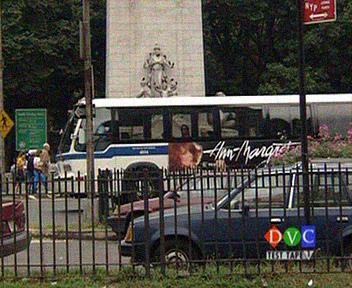
\includegraphics[trim=0cm 2cm 4cm 1cm, clip=true, width=0.3\textwidth]{figs/bus_nisy_s10_044.png}
		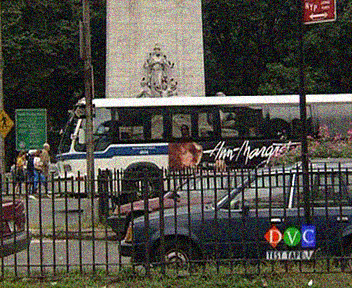
\includegraphics[trim=0cm 2cm 4cm 1cm, clip=true, width=0.3\textwidth]{figs/bus_nisy_s20_044.png}
		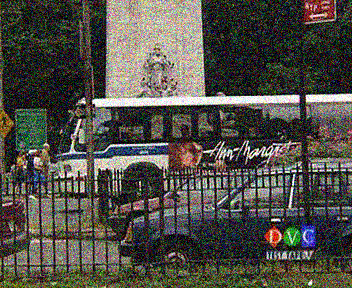
\includegraphics[trim=0cm 2cm 4cm 1cm, clip=true, width=0.3\textwidth]{figs/bus_nisy_s40_044.png}\\
		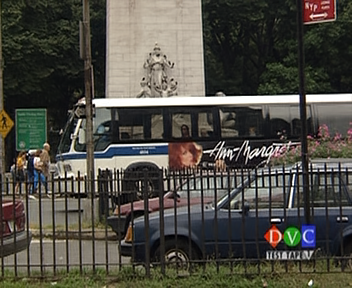
\includegraphics[trim=0cm 2cm 4cm 1cm, clip=true, width=0.3\textwidth]{figs/bus_vnlb_s10_tr2_044.png}
		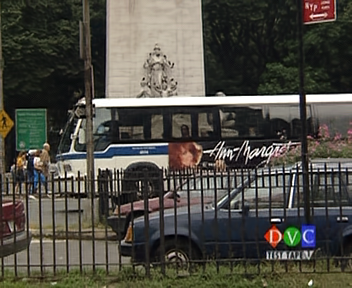
\includegraphics[trim=0cm 2cm 4cm 1cm, clip=true, width=0.3\textwidth]{figs/bus_vnlb_s20_tr2_044.png}
		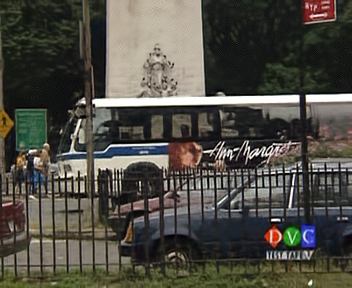
\includegraphics[trim=0cm 2cm 4cm 1cm, clip=true, width=0.3\textwidth]{figs/bus_vnlb_s40_tr2_044.png}\\
		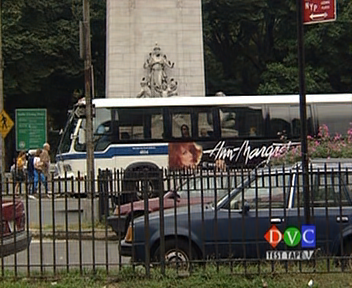
\includegraphics[trim=0cm 2cm 4cm 1cm, clip=true, width=0.3\textwidth]{figs/bus_s10_bm4d_044.png}
		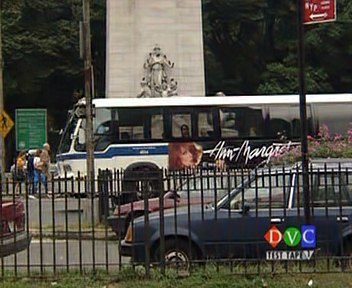
\includegraphics[trim=0cm 2cm 4cm 1cm, clip=true, width=0.3\textwidth]{figs/bus_s20_bm4d_044.png}
		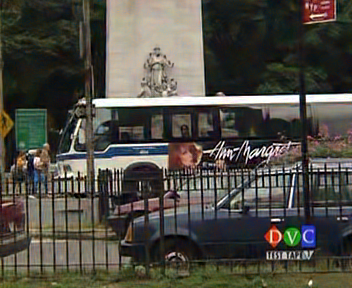
\includegraphics[trim=0cm 2cm 4cm 1cm, clip=true, width=0.3\textwidth]{figs/bus_s40_bm4d_044.png}\\
		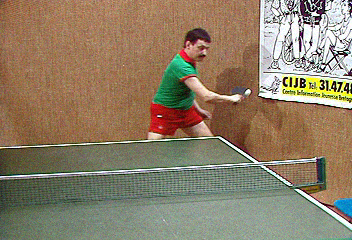
\includegraphics[trim=3.5cm 2cm 1.5cm .5cm, clip=true, width=0.3\textwidth]{figs/tennis_nisy_s10_140.png}
		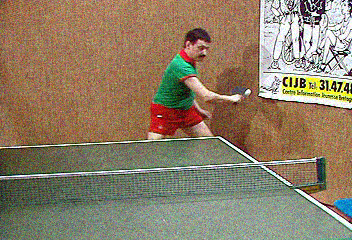
\includegraphics[trim=3.5cm 2cm 1.5cm .5cm, clip=true, width=0.3\textwidth]{figs/tennis_nisy_s20_140.png}
		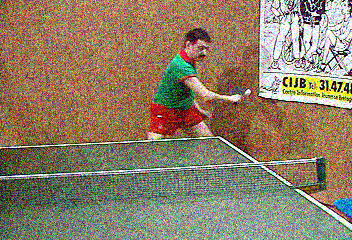
\includegraphics[trim=3.5cm 2cm 1.5cm .5cm, clip=true, width=0.3\textwidth]{figs/tennis_nisy_s40_140.png}\\
		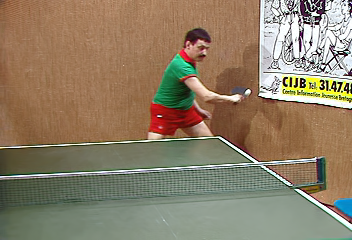
\includegraphics[trim=3.5cm 2cm 1.5cm .5cm, clip=true, width=0.3\textwidth]{figs/tennis_vnlb_s10_tr2_140.png}
		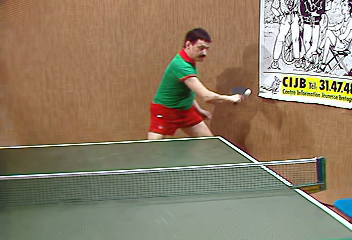
\includegraphics[trim=3.5cm 2cm 1.5cm .5cm, clip=true, width=0.3\textwidth]{figs/tennis_vnlb_s20_tr2_140.png}
		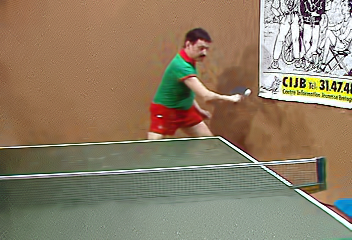
\includegraphics[trim=3.5cm 2cm 1.5cm .5cm, clip=true, width=0.3\textwidth]{figs/tennis_vnlb_s40_tr2_140.png}\\
		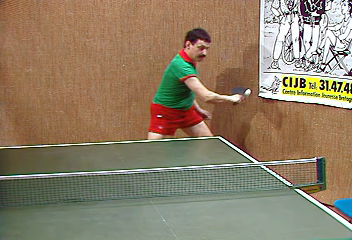
\includegraphics[trim=3.5cm 2cm 1.5cm .5cm, clip=true, width=0.3\textwidth]{figs/tennis_s10_bm4d_140.png}
		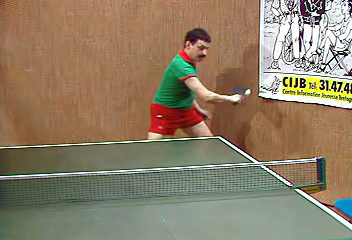
\includegraphics[trim=3.5cm 2cm 1.5cm .5cm, clip=true, width=0.3\textwidth]{figs/tennis_s20_bm4d_140.png}
		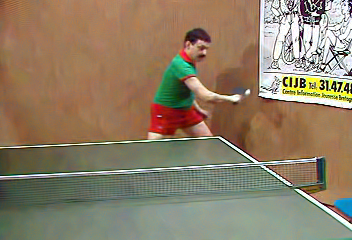
\includegraphics[trim=3.5cm 2cm 1.5cm .5cm, clip=true, width=0.3\textwidth]{figs/tennis_s40_bm4d_140.png}
	\end{center}
	\caption{Comparison of results obtained with VNLB ($n_t =5$) and V-BM4D-np.
	The first three rows, correspond to a frame of the bus sequence. From top to
	bottom: noisy input data. The last three rows correspond to the tennis sequence.
	Each column shows results obtained for $\sigma = 10$, $20$ and $40$.}
	\label{fig:results}
\end{figure}

\subsection{Implementation details}

\paragraph{Handling of color.} Color videos are handled as in \cite{Lebrun2013a}.
%
In the first stage, we express the video in a luminance-chrominance colorspace,
specifically we apply the opponent color transform (see \cite{Dabov2007tip,Lebrun2013a}).
Patch distances are computed using the luminance only. Using the 
$N_{\text{sim}}$ most similar patches, a group is built for each channel. These
groups are filtered independently (a Gaussian model is learnt for each of them).
%
In the second stage, the patch distance is computed using the RGB patches, and
a single \textit{a priori} Gaussian model is built for the each set
of similar RGB patches. 

\paragraph{Variance correction factor.} In practice, when computing the MAP
estimate by eq. \eqref{eq:map}, we introduce a parameter $\beta$ (with $\beta \approx 1$) multiplying
$\sigma^2I$ to be able to control the amount of filtering.

\paragraph{Patch distance threshold.} When building the group of similar
patches during the second stage, more than $N_{\text{sim}}$ patches are allowed
if their distances with respect to the reference patch are smaller than a
threshold $\tau$.  As in \cite{Lebrun2013ipol}, we set $\tau = 4$ (the distance between
patches is normalized by the number of elements in the patch and the number of
channels).

\paragraph{Speed-ups.} To accelerate the computation we apply two tricks
considered in \cite{Lebrun2013ipol}. The first one visits a patch each $N_{\text{step}}$
patches (similar to \cite{Dabov2007tip}). The second trick consists on the following.
After filtering the patches in a group, these patches are not considered again
as reference patches for a group. This reduces the number of groups of patches
that need to be processed by a factor of $N_{\text{sim}}$.

\subsection{Selection of parameters}
\label{sec:parameters}

For the experiments shown in \S \ref{sec:results} we used the following 
parameters.
\begin{description}
	\item[Patch size:] In both stages, we fixed the patch size at $s = 5$. Better 
		results can be obtained with higher patch sizes, but the computational cost
		scales considerably (e.g. the inversion of the covariance matrix is of $O(s^6)$).
	\item[Number of similar patches:] For the first stage, we set
		$N^{(1)}_{\text{sim}} = 3s^2n_t$  (recall that $n_t$ is the temporal
		extend of the search region). For the second step we 
		found better results using fewer patches, thus we set $N^{(2)}_{\text{sim}} = 3/4 s^2n_t$.
	\item[Search region:] In both stages, we used $n_x = s^2/2$.
		For the temporal search region, we found a good trade-off
		between computational time and quality of the results for $n_t = 5$. 
	\item[Patch distance threshold:] When building the group of similar patches
		in the second stage, more than $N_{\text{sim}}$ patches are allowed if their 
		distances with respect to the reference patch are smaller than a threshold $\tau$.
		As in \cite{Lebrun2013ipol}, we set $\tau = 4$ (the distance between patches is normalized by 
		the number of elements in the patch and the number of channels).
\end{description}

% stage 1
%
% patch size $s = 5$
% spatial search region $n_x = 37$
% temporal search region $n_t = 0,3,5$
% number of similar patches $3 s^2 n_t$, 3/4 s^2 n_t$$
% beta $\beta = 1; 1.2$
% tau n/a $\tau = 16$  
% offset $= s/2$

% stage 2
%
% patch size 
% spatial search region
% temporal search region
% number of similar patches
% beta
% tau
% offset

\begin{table}[htp!]
	\begin{center}
	\renewcommand{\tabcolsep}{3mm}
	\renewcommand{\arraystretch}{1.0}
	\begin{tabular}{ c | l |c c c c}
		\hline
		\rule{0pt}{12pt}$\sigma$ & Method                  & Tennis       & Coastguard   & Foreman      & Bus          \\\hline
		\multirow{5}{*}{$10$} & V-BM4D \cite{Maggioni2012} & \best{36.42} & \best{37.27} &       37.92  &       36.23  \\
		                      & V-BM4D-mp                  &       35.90  &       36.30  &       37.21  &       35.38  \\
		                      & V-BM4D-np                  &       35.56  &       36.20  &       36.90  &       35.09  \\
		                      & V-BM3D                     &       36.04  &       36.82  &       37.52  &       34.96  \\
		                      & VNLB $n_t = 0$             &       34.43  &       36.70  &       37.21  &       35.58  \\
		                      & VNLB $n_t = 3$             &       35.04  &       37.19  &       37.88  &       36.19  \\
									 & VNLB $n_t = 5$             &       35.28  & \best{37.30} & \best{38.11} & \best{36.37} \\\hline
%									 
		\multirow{5}{*}{$20$} & V-BM4D \cite{Maggioni2012} & \best{32.88} & \best{33.61} & \best{34.62} & \best{32.27} \\
		                      & V-BM4D-mp                  &       31.98  &       32.44  &       33.70  &       31.34  \\
		                      & V-BM4D-np                  &       31.67  &       32.24  &       33.34  &       30.95  \\
		                      & V-BM3D                     &       32.54  &       33.39  &       34.49  &       31.03  \\
		                      & VNLB $n_t = 0$             &       30.65  &       32.70  &       33.64  &       31.39  \\
									 & VNLB $n_t = 3$             &       31.26  &       33.35  &       34.25  &       32.11  \\
									 & VNLB $n_t = 5$             &       31.49  & \best{33.55} &       34.45  & \best{32.35} \\\hline
%									 
		\multirow{5}{*}{$40$} & V-BM4D \cite{Maggioni2012} & \best{29.52} & \best{30.00} & \best{31.30} &       28.32  \\
		                      & V-BM4D-mp                  &       28.14  &       28.73  &       30.09  &       27.44  \\
		                      & V-BM4D-np                  &       27.97  &       28.43  &       29.69  &       27.02  \\
									 & V-BM3D                     &       29.20  & \best{29.99} &       31.17  &       27.34  \\
		                      & VNLB $n_t = 0$             &       27.43  &       28.88  &       30.15  &       27.60  \\
									 & VNLB $n_t = 3$             &       27.97  &       29.60  &       30.72  &       28.23  \\
									 & VNLB $n_t = 5$             &       28.11  &       29.78  &       30.82  & \best{28.40} \\\hline
	\end{tabular}
	\end{center}
	\caption{PSNRs obtained for the four classic color test sequences used in
	\cite{Maggioni2012}. See text for details.}
	\label{tab:psnr-classic}
\end{table}


\begin{table}[htp!]
	\begin{center}
	\renewcommand{\tabcolsep}{2mm}
	\renewcommand{\arraystretch}{1.0}
	\begin{tabular}{ c | l |c c c c c}
		\hline
		\rule{0pt}{12pt}$\sigma$ & Method     & Army & DogDance & Evergreen & Mequon & Walking  \\\hline
		\multirow{5}{*}{$10$} & V-BM4D-np      &       37.77  &       35.70  &       35.40  &       38.09  &       38.85  \\
		                      & VNLB $n_t = 0$ &       36.90  &       35.42  &       34.84  &       38.43  &       38.86  \\
		                      & VNLB $n_t = 3$ &       37.65  &       35.87  &       35.38  &       39.09  &       39.69  \\
									 & VNLB $n_t = 5$ & \best{37.88} & \best{36.01} & \best{35.53} & \best{39.20} & \best{39.74} \\\hline
%									                                                                                           
		\multirow{5}{*}{$20$} & V-BM4D-np      &       32.91  &       31.50  &       30.94  &       33.60  &       34.27  \\
		                      & VNLB $n_t = 0$ &       33.77  &       32.44  &       31.68  &       35.61  &       35.60  \\
									 & VNLB $n_t = 3$ &       34.45  &       32.90  &       32.15  &       35.89  &       36.12  \\
									 & VNLB $n_t = 5$ & \best{34.59} & \best{33.02} & \best{32.27} & \best{35.90} & \best{36.12} \\\hline
%									                                                                                           
		\multirow{5}{*}{$40$} & V-BM4D-np      &       30.42  &       29.29  &       28.65  &       31.02  &       31.64  \\
		                      & VNLB $n_t = 0$ &       30.55  &       29.41  &       28.66  &       31.78  &       31.86  \\
									 & VNLB $n_t = 3$ & \best{31.02} & \best{29.73} & \best{29.03} & \best{31.88} & \best{31.92} \\
									 & VNLB $n_t = 5$ & \best{31.06} & \best{29.74} & \best{29.08} &       31.70  &       31.74  \\\hline
	\end{tabular}
	\end{center}
	\caption{PSNRs obtained for the five color sequences from the Middlebury
	dataset \cite{middleburyOflow}. See text for details.}
	\label{tab:psnr-middlebury}
\end{table}

\section{Results}
\label{sec:results}

In this section we present preliminary results obtained with the proposed
method on the classic color test sequences \emph{tennis}, \emph{coastguard}, \emph{foreman},
\emph{bus}. In order to measure the effect of the additional temporal
dimension, we tested our method considering temporal search ranges of $1, 3$ and $5$ frames.
The results are shown in Table \ref{tab:psnr-classic}. The proposed method is labeled VNLB.
For these sequences, the best results were obtained with
$n_t = 5$ (two frames before and after the frame of the current patch). Larger 
values of $n_t$ do not necessarily lead to better results. One possible reason
for that is that our search does not take motion into account. As a
consequence, in the presence of motion, similar patches might exit of the
search range after a certain number of frames.

For comparison, we also show the result of V-BM3D and three versions of V-BM4D.
The method labeled V-BM4D-\cite{Maggioni2012} corresponds to the results reported
in \cite{Maggioni2012}. The results labeled V-BM4D-np and V-BM4D-mp were
obtained using the implementation available online \cite{bm4dcode}. This
implementation provides three parameter profiles of increasing quality and
complexity: ``low complexity profile'', ``normal profile'' and ``modified
profile''. We show the results obtained with the normal (V-BM4D-np) and
modified (V-BM4D-mp) profiles.
Let us note that the normal profile has a
computation time comparable to our method. Running with a
single core in a Intel Xeon X7560 (2.27GHz) CPU, 
our current implementation takes on average $10s$ per frame for a video of CIF
resolution ($352\times288$). V-BM4D takes $13s$ per frame with the normal
profile and $44s$ with the modified profile.

In terms of PSNR, the best results for these sequences is obtained by
V-BM4D-\cite{Maggioni2012}. Our method seems to do better for $\sigma = 10$,
and for the bus sequence, and has problems with the tennis sequence. For
$\sigma = 20$ and $40$ our method performs similar to V-BM3D (except for the
tennis sequence). 

We also show quantitative results obtained in for some sequences from the
optical flow Middlebury dataset (the sequences have 8 frames each), and compare
agaist V-BM4D-np (see table \ref{tab:psnr-middlebury}. For these sequences, the
proposed method outpeforms V-BM4D-np. 

For a qualitative analysis we show in Figure \ref{fig:results} results obtained
with nonlocal Bayes (setting $n_t = 5$) and V-BM4D-np. Interestingly, for $\sigma = 20$
and $40$, V-BM4D-np is able to better recover the wallpaper texture in tennis,
but does worse than VNLB for the foliage texture of the trees in bus. 
%One
%plausible reason for this is that the spatial bi-orthogonal wavelets and
%DCT transforms used by BM4D are very well suited to the structured pattern of the
%wallpaper.
For high levels of noise, the wallpaper texture is masked by the noise. 
It is possible that when comparing 2D patches the noise dominates in the
comparison. Using spatio-temporal volumes reduces the distance noise,
allowing to find similar patches with the same regular texture pattern.

For $\sigma = 40$ the VNLB method exhibits some noise in flat or over-smoothed
regions (e.g. wallpaper in tennis sequence). It seems that the
Wiener filter of eq. \eqref{eq:map} is not aggressive enough for this noise level.

% \textcolor{red}{ 
% An important aspect of the quality of any video processing algorithm is the 
% temporal consistency of the result. The proposed method does not enforce
% temporal consistency. To visualize that we compute the absolute value of the 
% time difference between two successive frames of the estimated video:
% \[d(x,t) = \|\widetilde{u}(x,t) - \widetilde{u}(x,t+1)\|.\]
% Figure shows the results obtained by averaging $d(x,t)$ for four consecutive
% frames in the tennis sequence for V-BM4D-np and VNLB, with $n_t =5$. Since the camera
% is static one should expect a low value of the difference in the walls and the table.
% The result of VNLB shows higher values than V-BM4D (in the figure the
% differences were computed between the luminance channel and the white
% represents a difference of 20 levels.}
% 
% \begin{figure}[thpb!]
% 	\begin{center}
% 		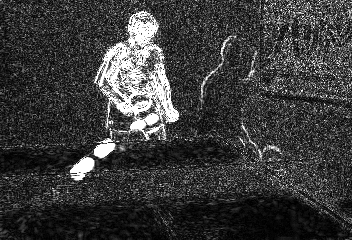
\includegraphics[trim=3.5cm 2cm 1.5cm .5cm, clip=true, width=0.3\textwidth]{figs/time_diff_vnlb_s10.png}
% 		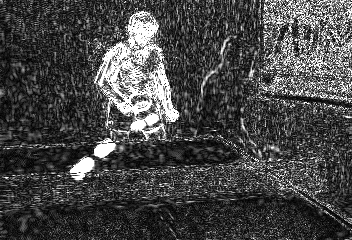
\includegraphics[trim=3.5cm 2cm 1.5cm .5cm, clip=true, width=0.3\textwidth]{figs/time_diff_vnlb_s20.png}
% 		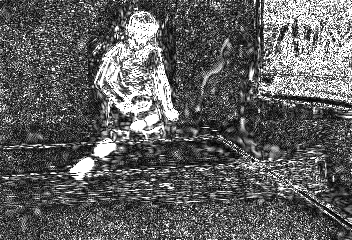
\includegraphics[trim=3.5cm 2cm 1.5cm .5cm, clip=true, width=0.3\textwidth]{figs/time_diff_vnlb_s40.png}\\
% 		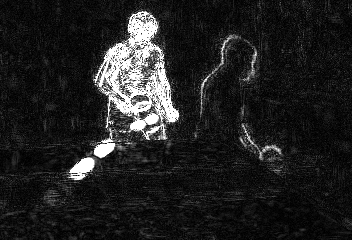
\includegraphics[trim=3.5cm 2cm 1.5cm .5cm, clip=true, width=0.3\textwidth]{figs/time_diff_bm4d_s10.png}
% 		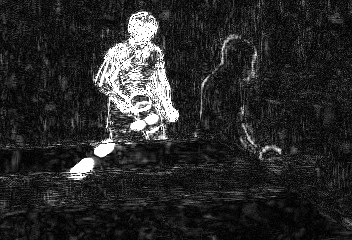
\includegraphics[trim=3.5cm 2cm 1.5cm .5cm, clip=true, width=0.3\textwidth]{figs/time_diff_bm4d_s20.png}
% 		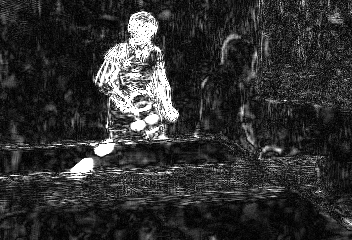
\includegraphics[trim=3.5cm 2cm 1.5cm .5cm, clip=true, width=0.3\textwidth]{figs/time_diff_bm4d_s40.png}
% 	\end{center}
% 	\caption{\textcolor{red}{Temporal coherency of the denoising. Average absolute value of time difference
% 	between five successive frames of the denoising result for tennis  with
% 	$\sigma=20$ (the time difference was computed between the luminance
% 	channels). Top row corresponds to VNLB ($n_t =2$) and bottom
% 	V-BM4D-np. The columns correspond to noise of level $\sigma = 10, 20, 40$.
% 	Darker values means lower average time difference.}} \label{fig:time-diff}
% \end{figure}

% \begin{table}
% 	\begin{center}
% 	\renewcommand{\tabcolsep}{3mm}
% 	\renewcommand{\arraystretch}{1.3}
% 	\begin{tabular}{ c | c |c c c c}
% 		\hline
% 		\rule{0pt}{12pt}$\sigma$ & Method     & Tennis       & Coastguard   & Foreman      & Bus          \\\hline
% 		\multirow{5}{*}{$10$} & V-BM4D        & \best{36.42} & \best{37.27} &       37.92  & \best{36.23} \\
% 		                      & V-BM3D        &       36.04  &       36.82  &       37.52  &       34.96  \\
% 		                      & VNLB $n_t = 0$ &       32.13  &       33.75  &       34.60  &       32.71  \\
% 		                      & VNLB $n_t = 3$ &       35.12  &       37.20  &       37.89  &       36.14  \\
% 									 & VNLB $n_t = 5$ &       35.19  & \best{37.26} & \best{38.00} &       36.11  \\\hline
% %									 
% 		\multirow{5}{*}{$25$} & V-BM4D        & \best{32.88} & \best{33.61} & \best{34.62} & \best{32.27} \\
% 		                      & V-BM3D        &       32.54  &       33.39  &       34.49  &       31.03  \\
% 		                      & VNLB $n_t = 0$ &       30.58  &       32.47  &       33.44  &       31.26  \\
% 									 & VNLB $n_t = 3$ &       31.22  &       33.39  &       34.28  &       32.01  \\
% 		                      & VNLB $n_t = 5$ &       31.25  &       33.44  &       34.34  &       31.94  \\\hline
% %									 
% 		\multirow{5}{*}{$40$} & V-BM4D        & \best{29.52} & \best{30.00} & \best{31.30} & \best{28.32} \\
% 		                      & V-BM3D        &       29.20  &       29.99  &       31.17  &       27.34  \\
% 		                      & VNLB $n_t = 0$ &       27.24  &       28.55  &       29.74  &       27.37  \\
% 									 & VNLB $n_t = 3$ &       27.96  &       29.68  &       30.85  &       28.17  \\
% 									 & VNLB $n_t = 5$ &       28.02  &       29.76  &       30.94  &       28.14  \\\hline
% 	\end{tabular}
% 
% 	\bigskip
% 	\end{center}
% 	\caption{PSNR for sequences taken from the Middlebury optical flow benchmark.}
% \end{table}


\section{Conclusions}
\label{sec:conclusion}

We presented a Bayesian video denoising algorithm assuming a Gaussian model for similar patches. 
We show preliminary results and compare it with two methods from the
state-of-the-art, V-BM3D and V-BM4D.
The resulting method does not require motion estimation.%, and as such it shows
%lower temporal coherency than V-BM4D.
In terms of PSNR
the results obtained show state-of-the-art performance for low levels of noise.
For higher levels of noise the performance is comparable to V-BM3D and improves
over the default version of V-BM4D.


%
% ---- Bibliography ----
%

\bibliography{image_denoising.bib,video_denoising.bib}
\bibliographystyle{splncs03}

\end{document}
